\documentclass[a4paper,11pt,landscape,twocolumn]{article}

\usepackage{../préambule}
\usepackage{clipboard}
\usetikzlibrary{calc}

\newcommand{\myAdd}[2]{\directlua{tex.print(#1 + #2)}}

\begin{luacode}
	function print_items(points)
		for _, p in ipairs(points) do
			tex.sprint("\\item (", p.x, "; ", p.y, ")")
		end
	end

	function print_path(points)
		tex.sprint("\\draw[red,thick] ")
		for i, p in ipairs(points) do
		 	if i ~= 1 then
		 		tex.sprint(" -- ")
		 	end
		 	tex.sprint("(", p.x * 2 + 3.5, ",", p.y * 2 + 2.5, ")")
		end
		tex.sprint(";")
	end
\end{luacode}

\begin{document}

\Copy{beta}{
	\directlua{
		points = {
				{ x = -1.5, y = -1.5 },
				{ x = -1.5, y = -1 },
				{ x = -0.5, y = -1 },
				{ x = -0.5, y = -0.5 },
				{ x = -1, y = -0.5 },
				{ x = -1, y = 1 },
				{ x = 0, y = 1 },
				{ x = 0, y = 0.5 },
				{ x = 1.5, y = 0.5 },
				{ x = 1.5, y = 0 },
				{ x = 0.5, y = 0 },
				{ x = 0.5, y = -0.5 },
				{ x = 2, y = -0.5 },
			}
	}

	{\large \textbf{Coordonnées β :}}
	\begin{multicols}{2}
		\begin{enumerate}[label={\Alph*}]
			\directlua{print_items(points)}
		\end{enumerate}
	\end{multicols}

	\vspace{2em}
	\hrule
	\vspace{2em}

	\textbf{Labyrinthe β :} \vspace{1em}

	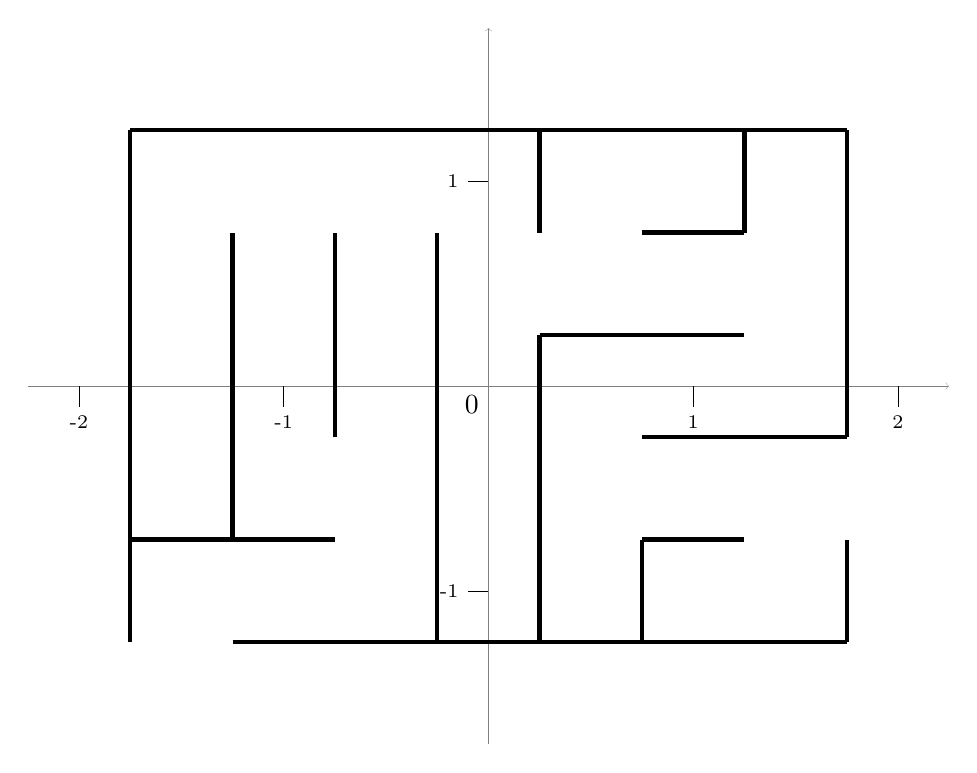
\begin{tikzpicture}[scale=1.3]
		\draw[gray,ultra thin,->] (-1,2.5) -- (8,2.5);
		\draw[gray,ultra thin,->] (3.5,-1) -- (3.5,6);
		\node[below left] at (3.5,2.5) {0};

		\draw[very thin] (-0.5,2.5) -- (-0.5,2.3) node[below] {\scriptsize -2};
		\draw[very thin] (1.5,2.5) -- (1.5,2.3) node[below] {\scriptsize -1};
		\draw[very thin] (5.5,2.5) -- (5.5,2.3) node[below] {\scriptsize 1};
		\draw[very thin] (7.5,2.5) -- (7.5,2.3) node[below] {\scriptsize 2};

		% \draw[very thin] (3.5,-1.5) -- (3.3,-1.5);
		\draw[very thin] (3.5,0.5) -- (3.3,0.5) node[left] {\scriptsize -1};
		\draw[very thin] (3.5,4.5) -- (3.3,4.5) node[left] {\scriptsize 1};
		% \draw[very thin] (3.5,6.5) -- (3.3,6.5);

		\foreach \xa/\ya/\xb/\yb in {
				0/0/0/5,
				1/0/7/0,
				0/5/7/5,
				7/0/7/1,
				7/2/7/5,
				0/1/2/1,
				1/1/1/4,
				2/2/2/4,
				3/0/3/4,
				4/4/4/5,
				4/0/4/3,
				4/3/6/3,
				5/0/5/1,
				5/1/6/1,
				5/2/7/2,
				6/5/6/4,
				6/4/5/4
			} {
				\draw[ultra thick] (\xa,\ya) -- (\xb,\yb);
			}

		% \directlua{print_path(points)}
	\end{tikzpicture}
}

\newpage

\Paste{beta}

\end{document}